
%(BEGIN_QUESTION)
% Copyright 2012, Tony R. Kuphaldt, released under the Creative Commons Attribution License (v 1.0)
% This means you may do almost anything with this work of mine, so long as you give me proper credit

A vessel containing a pressurized gas will experience an upward force ($F$) exerted on its lid by the gas pressure ($P$), equal to the product of gas pressure and lid area ($F = PA$).  The pressure of the gas inside of any sealed vessel may be predicted by the Ideal Gas Law relating pressure to vessel volume, gas quantity, and gas temperature ($PV = nRT$):

$$\includegraphics[width=15.5cm]{i03035x01.eps}$$

\vskip 10pt

Suppose we wished to have a single formula for calculating force on the lid of a vessel given all the other factors (gas quantity $n$, lid area $A$, gas temperature $T$, vessel volume $V$, and the gas law constant $R$).  Combine the force-pressure-area formula ($F = PA$) and the Ideal Gas Law formula ($PV = nRT$) in order to arrive at this new formula solving for $F$ in terms of all the other variables:

\vskip 20pt

$F =$

\vskip 20pt

\underbar{file i03035}
%(END_QUESTION)





%(BEGIN_ANSWER)

 
%(END_ANSWER)





%(BEGIN_NOTES)

Manipulating the Ideal Gas Law to solve for $P$:

$$PV = nRT$$

$$P = {nRT \over V}$$

\vskip 10pt

Substituting this definition for $P$ into the force-pressure-area formula:

$$F = PA$$

$$F = \left( {nRT \over V} \right) A$$

\vskip 10pt

Simplifying:

$$F = {AnRT \over V}$$

%INDEX% Mathematics review: manipulating and combining equations to form a new equation

%(END_NOTES)


